\documentclass[12pt]{article}

% Preamble

\usepackage[margin=1in]{geometry}
\usepackage{amsfonts, amsmath, amssymb}
\usepackage{fancyhdr, float, graphicx}
\usepackage[utf8]{inputenc} % Required for inputting international characters
\usepackage[T1]{fontenc} % Output font encoding for international characters
\usepackage{fouriernc} % Use the New Century Schoolbook font
\usepackage[nottoc, notlot, notlof]{tocbibind}
\usepackage{url}
\usepackage{placeins}
\usepackage{multirow}
% Header and Footer
\pagestyle{fancy}
\fancyhead{}
\fancyfoot{}
\fancyhead[L]{\textit{\Large{Experiment 7}}}
\fancyhead[R]{\textit{something}}
\fancyfoot[C]{\thepage}
\renewcommand{\footrulewidth}{1pt}



% Other Doc Editing
\parindent 0ex
\renewcommand{\baselinestretch}{1}

\begin{document}
	
	\begin{titlepage} 
		\centering 
		
		%---------------------------NAMES-------------------------------
		
		\huge\textsc{
			MIT World Peace University
		}\\
	
		\vspace{0.75\baselineskip} % space after Uni Name
		
		\LARGE{
			Physics\\
			First Year B. Tech, Trimester 3\\
			Academic Year 2021-22
		}
		
		\vfill % space after Sub Name
		
		%--------------------------TITLE-------------------------------
		
		\rule{\textwidth}{1.6pt}\vspace*{-\baselineskip}\vspace*{2pt}
		\rule{\textwidth}{0.6pt}
		\vspace{0.75\baselineskip} % Whitespace above the title
		
		
		
		\huge{\textsc{
				Characteristics of a Solar Cell
			}} \\
		
		
		
		\vspace{0.5\baselineskip} % Whitespace below the title
		\rule{\textwidth}{0.6pt}\vspace*{-\baselineskip}\vspace*{2.8pt}
		\rule{\textwidth}{1.6pt}
		
		\vspace{1\baselineskip} % Whitespace after the title block

		%--------------------------SUBTITLE --------------------------	
			
		\LARGE\textsc{
			Experiment No. 7
		} % Subtitle or further description
		\vfill
		
		%--------------------------AUTHOR-------------------------------
		
		Prepared By
		\vspace{0.5\baselineskip} % Whitespace before the editors
		
		\Large{
			109054. Krishnaraj Thadesar
			
			Division 9 Batch I3
		}
		
		
		\vspace{0.5\baselineskip} % Whitespace below the editor list
		\today

	\end{titlepage}

	\begin{center}
	{\Large Pledge}\\
	\vspace{0.5cm}
	I solemnly affirm that I am presenting this journal based on my own experimental work. I have neither copied the observations, calculations, graphs and results from others nor given it to others for copying.\\
		\end{center}
	
	\vspace{0.5cm}
	
    \begin{flushright}
	{\large Signature of the student}\\
	\vspace{1cm}
	 \end{flushright}
	
	\section{Aim}
	\noindent
	To plot I-V characteristics of solar cell, to determine its fill factor and corresponding
	optimum load
	
\section{Apparatus}


		\begin{enumerate}
			\item Solar cell/solar panel
			\item Current and voltmeters (OR DMM)
			\item Variable load and source of light
		\end{enumerate}

\section{Significance of the Experiment}
	\textit{Solar cell is a specially designed PN junction which converts
	light in to electrical power. The ability of the solar cell to deliver optimum power to the
	optimized load is signified in terms of it’s fill factor. The present experiment aims at calculation
	of the fill factor and corresponding optimum load for a given solar cell.}
	
\section{Theory}
Solar cell is a specially designed PN junction diode that converts light into electrical
power. This conversion occurs in three stages. When the PN junction is exposed to light, electron
	hole pairs are generated in P and N regions. These are then separated across opposite electrodes
	due to emf at the junction. (refer Fig.7.1). The separated carriers accumulate across the metal
	contacts and thus generate a potential difference (p.d). This p.d. can drive the optically excited
	minority carriers in circuit. Thus solar cell, when exposed to light, behaves as a battery that can
	deliver power to a load. The typical voltage and current from one junction is around 0.6 volts and
	a few micoramp, however this can be increased by cascading the solar cells in series and parallel
	(solar panels). Solar cells generate electricity from inexhaustible, freely available sunlight and
	without pollution, without accidents and need less maintenance. Further, an option of
	decentralized production can decrease transmission losses. However the low efficiency (10%),
	high production cost and dependence on sunlight limit its applications to remote areas (such as
	satellites and villages in deserts, forests) and low power accessories (such as calculators, wrist
	watches, street lights and solar water pumps). If efficiency is improved, solar power may find
	uses in solar automobiles, solar houses and many other areas.
	\begin{figure}[H]
		\centering
		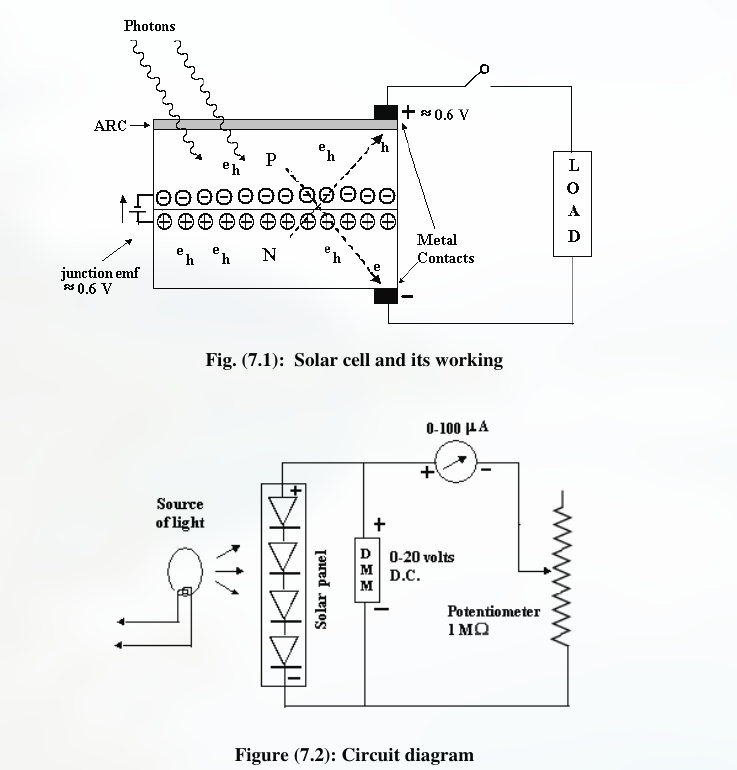
\includegraphics[scale=0.8]{thoeryfi.png}
		\label{it}
	\end{figure}

\section{Procedure}
\begin{enumerate}
	 
	\item Connect the circuit as shown in the diagram (Fig.8.2) and get it checked. Connect DMM as a 0-20 voltmeter in parallel and DMM and $0-200 \mu \mathrm{A}$ in series across the $1 \mathrm{M} \Omega$ variable load.
	\item Make the light source ON and keep it to optimum intensity.
	\item Take as many as possible current and voltage readings by varying the load. The readings corresponding to minimum and maximum load must be taken. Tabulate your observations as per table $8.1$
	\item Plot the graph of current Vs voltage. This represents characteristics of solar cell (refer Fig 8.3)
	\item Extrapolate the graph on current and voltage axis. While extrapolating the curve keep the slope same. Calculate $I_{S C}$ (Short circuit current) and $V_{O C}$ (Open circuit voltage) from the intercept of the curve on current and voltage axis respectively. Draw perpendiculars at $I_{S C}$ and $V_{O C}$. Intersection of these two lines defines a point $P_{I}\left(I_{S C,}, V_{O C}\right)$. The product $P_{I}=$ $I_{S C} \times V_{O C}$ signifies ideal but unachievable power (refer Fig.8.3). The ideal power is unachievable because short circuit condition and open circuit condition cannot be obtained simultaneously.
	\item An intersection of a line joining origin $(0,0)$ to $P_{I}\left(I_{S C}, V_{O C}\right)$ on the curve gives a point, $P_{W}\left(I_{W}, V_{W}\right)$, where current and voltage are simultaneously optimum. The product $P_{W}=I_{W} \times V_{W}$ thus signifies the optimum and realizable and hence workable power. Measure $I_{W}$ and $V_{W}$ and calculate workable power $\left(P_{W}\right)$
	\item Calculate the fill factor $\left(f=\frac{P_{W}}{P_{I}} \times 100 \%\right)$. The fill factor signifies the extent to which workable power is close to ideal power. Alternatively, it signifies the extent to which workable power rectangle 'fills' the ideal power rectangle.
	\item Calculate the workable load $R_{W}=\frac{V_{W}}{I_{W}} . R_{W}$ signifies the workable load at which solar cell can deliver optimum/workable power.
	\item Tabulate your calculations and results as per the table (8.2)
\end{enumerate}

\section{Observations}

\begin{figure}[H]
	\centering
	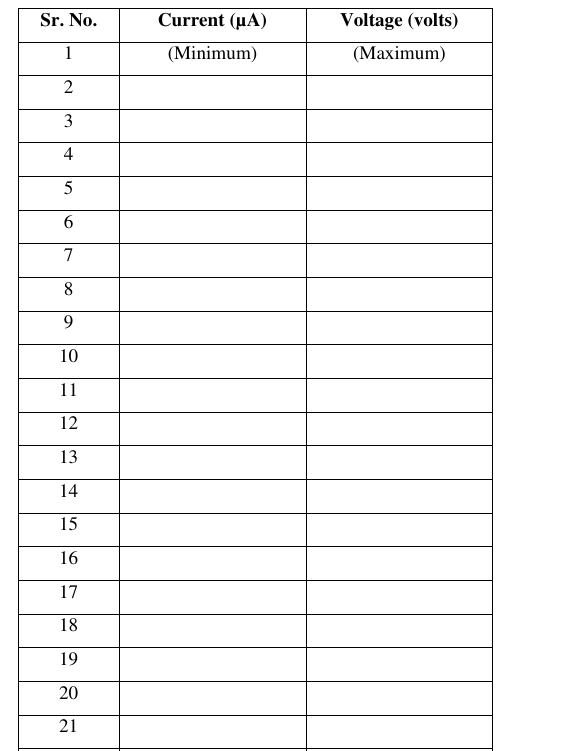
\includegraphics[scale=0.9]{obs.png}
	\label{it}
\end{figure}

\section{Calculations}

\begin{figure}[H]
	\centering
	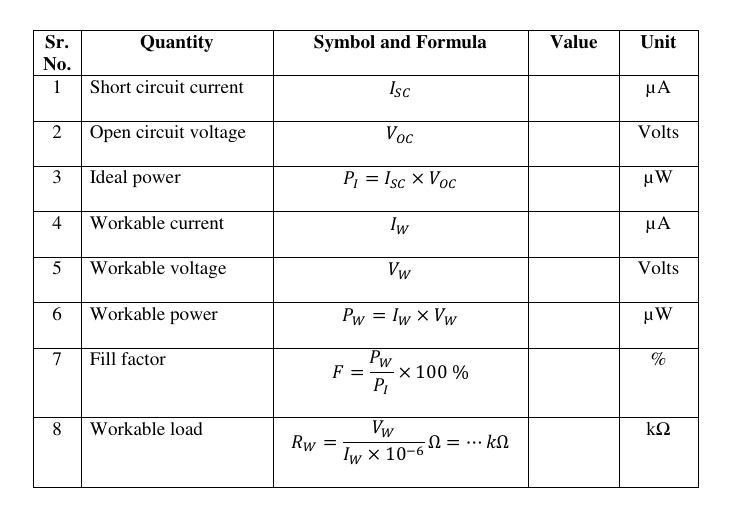
\includegraphics[scale=0.9]{calc2.png}
	\label{it}
\end{figure}

\section{Graphs}
\subsection{Plot between Volts and Current in Micro Amperes}
\begin{figure}[H]
	\centering
	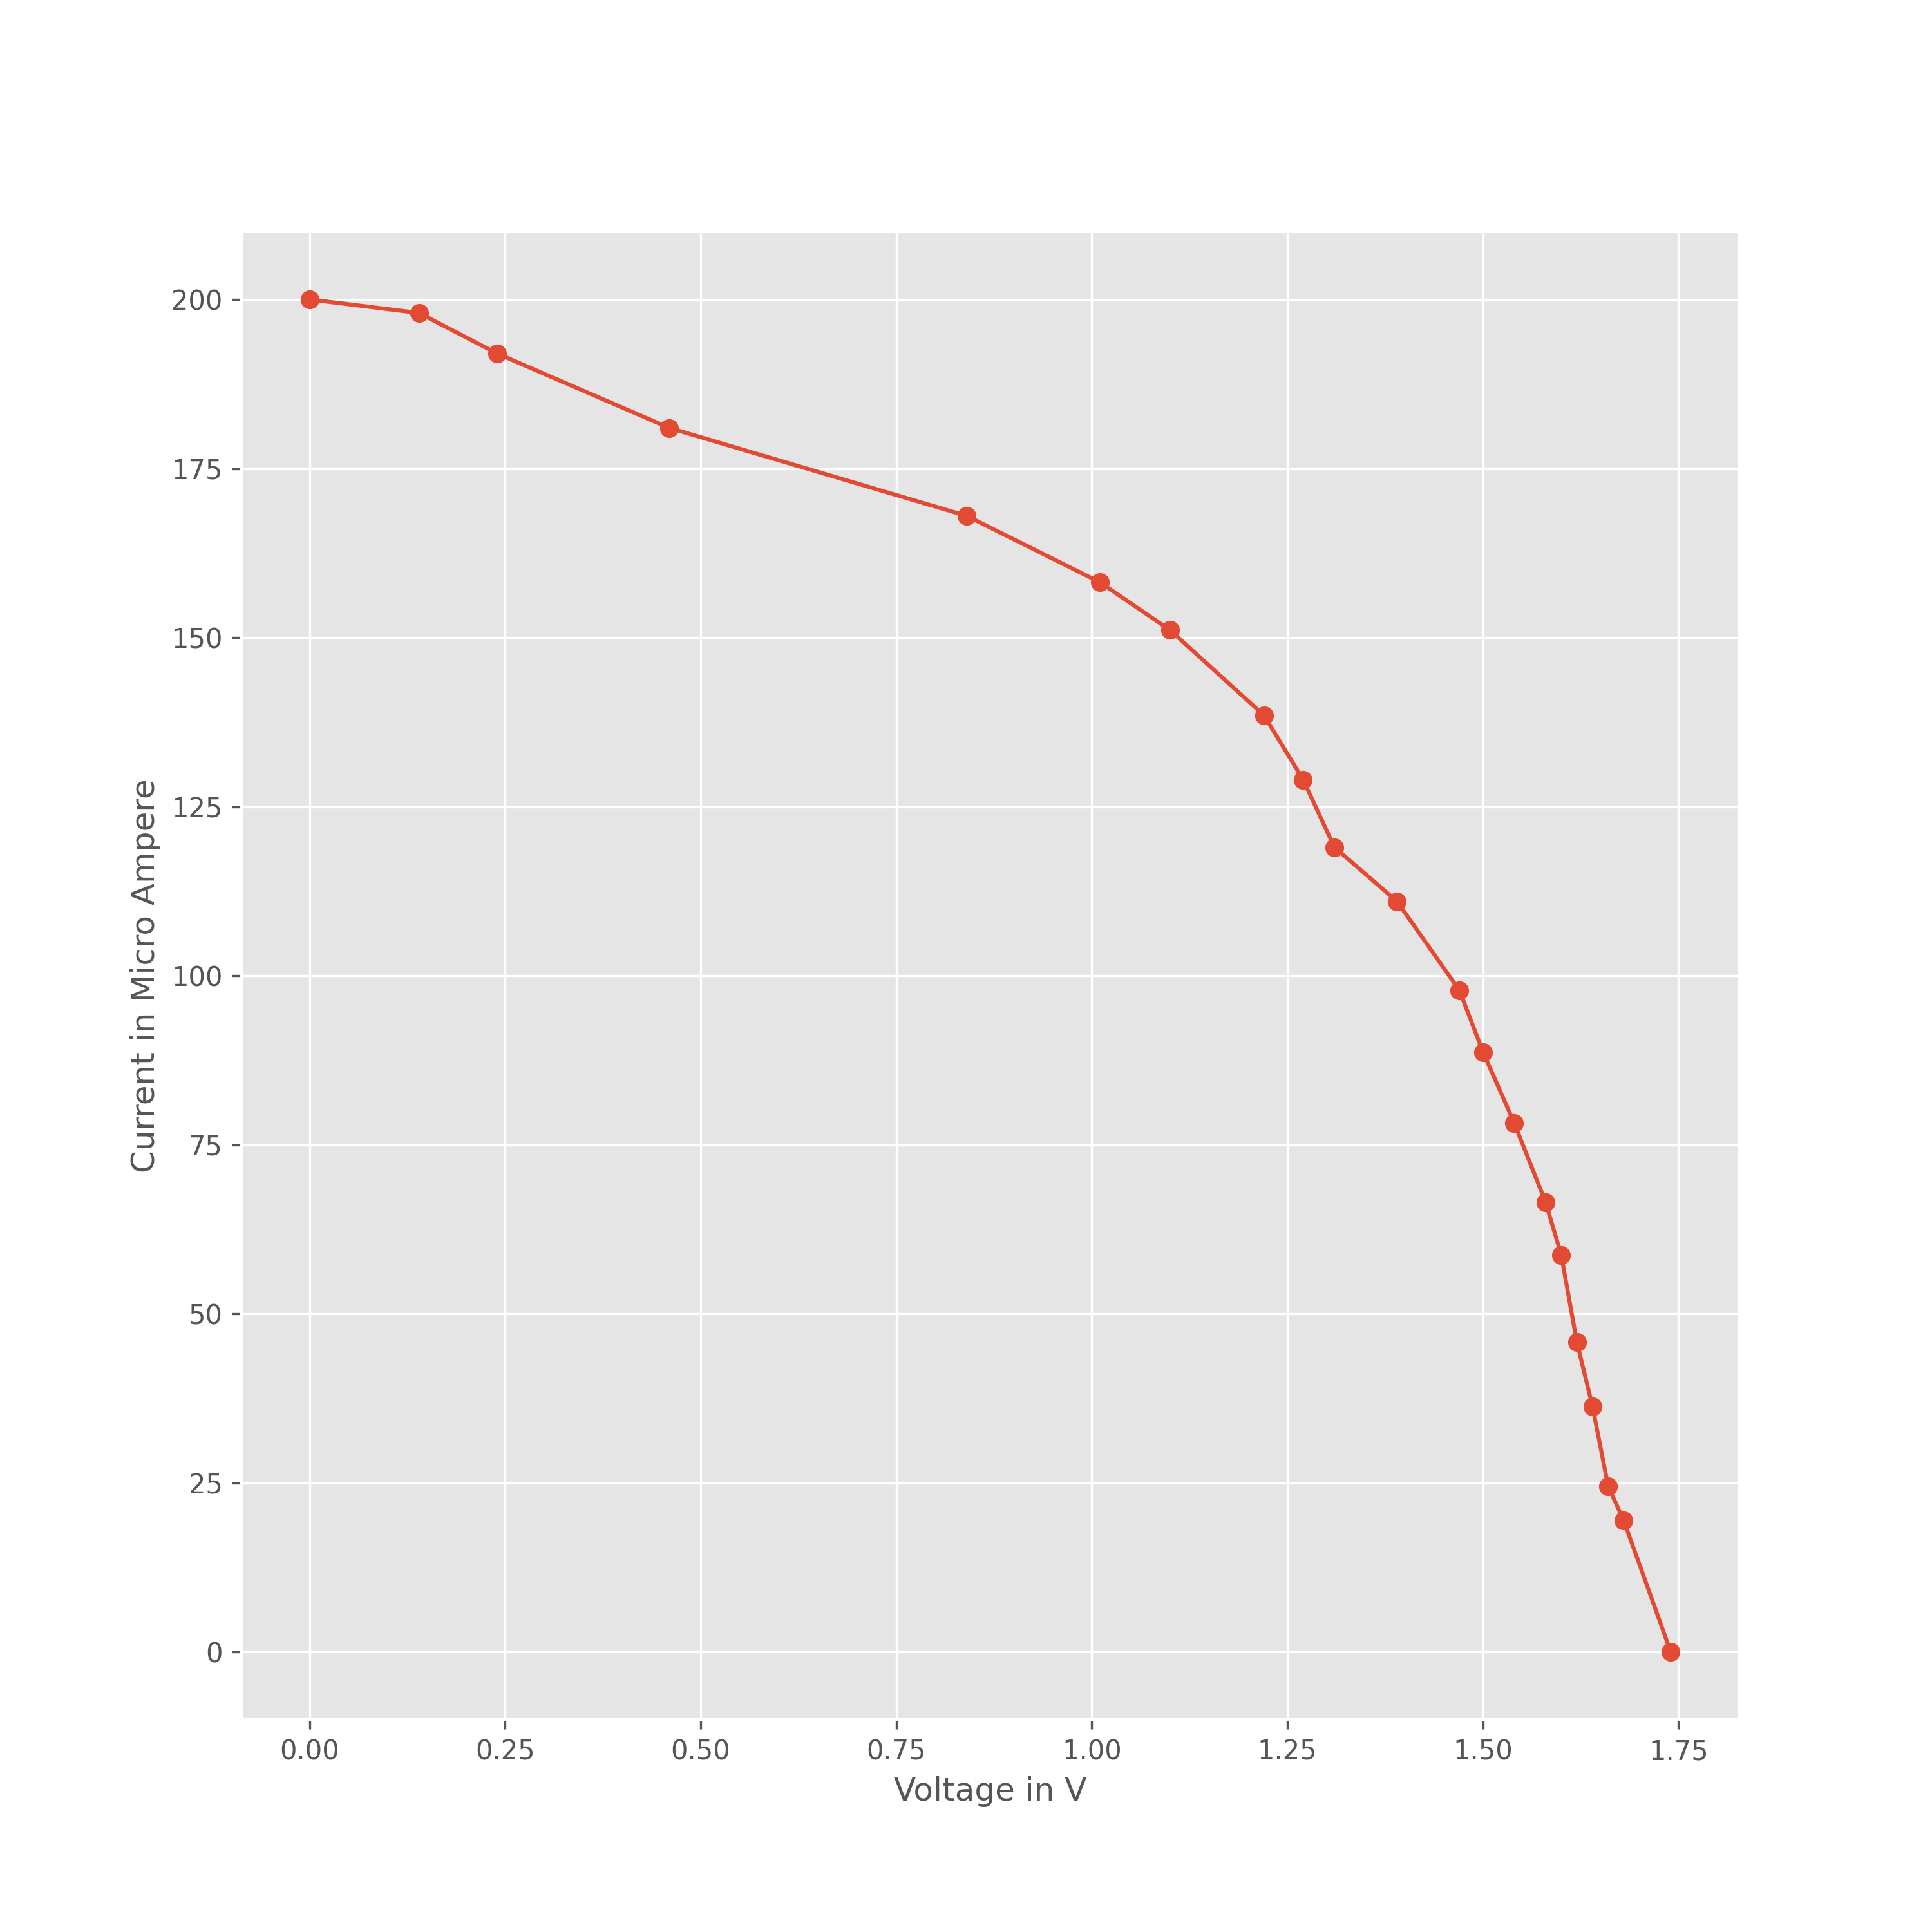
\includegraphics[scale=0.6]{fig.png}
	\label{it}
\end{figure}


\section{My Understanding of the Experiment}
A solar cell is a special pn junction diode that converts light into electrical power. As photons hit the cell, it excites their electrons, thereby producing electricity.
In the process, some energy is wasted. An extent of how much power is wasted is given by the cell's Fill factor. As the working power is less than the ideal power. 
It is that fill factor that we wish to calculate in this experiment. If this fill factor is improved, and if the efficiency of the cell also improves significantly, solar cells are a very promising candidate in renewable energy. 
\end{document}